%==================================================
%  From Keldysh to Lévy — Unified EM Noise Framework
%==================================================
\documentclass[11pt,a4paper]{article}

%------------------- Packages ---------------------
\usepackage[utf8]{inputenc}
\usepackage[T1]{fontenc}
\usepackage{lmodern}
\usepackage{amsmath, amssymb, amsfonts}
\usepackage{graphicx}
\usepackage{booktabs}
\usepackage{tabularx}
\usepackage{physics}
\usepackage{siunitx}
\usepackage{authblk}
\usepackage{csquotes}
\usepackage[most]{tcolorbox}
\usepackage{tikz}
\usetikzlibrary{patterns,decorations.pathmorphing,arrows.meta,positioning,calc}
\usepackage{hyperref}

\hypersetup{
  colorlinks = true,
  linkcolor = blue,
  citecolor = blue,
  urlcolor  = blue
}

%------------------- Metadata ---------------------
\title{From Keldysh to L\'evy:\\
  A Unified Framework for Electromagnetic Noise in Trapped Ions}

\author[1]{Ulrich Warring, et al.}
\affil[1]{Physikalisches Institut, Universität Freiburg, Germany}

\date{\today}

%------------------- Document ---------------------
\begin{document}
\maketitle

\begin{abstract}
We present a framework connecting microscopic descriptions of electromagnetic noise
from the Keldysh formalism to L\'evy-statistics-based macroscopic noise models.
The goal is to provide a unified language for analyzing fluctuating fields
that affect trapped-ion motion and internal coherence,
bridging theory, scattering models, and experimental inference through a
common description of motional decoherence encompassing both heating and
dephasing channels.
\end{abstract}

%------------------- Section Includes --------------
\section{Introduction}

Trapped ions are sensitive probes of electromagnetic fields and their fluctuations. Understanding and mitigating motional decoherence—the degradation of quantum coherence in the ion's harmonic motion—has been central to quantum information processing and precision spectroscopy since the earliest experiments~\cite{Turchette2000,Wineland1998}. 

Motional decoherence encompasses two physically distinct channels. \emph{Heating} exchanges energy with the environment through resonant force fluctuations near the trap frequency $\omega_t$, increasing the mean phonon number $\langle n \rangle$ and reducing motional state purity. \emph{Dephasing} arises from slow variations in the trapping potential or stray fields that modulate the instantaneous frequency $\omega_t \to \omega_t + \delta\omega(t)$, producing random phase evolution $\phi(t) = \int_0^t \delta\omega(t') dt'$ without energy exchange. Both processes degrade the fidelity of motional quantum states, but they are controlled by different parts of the noise spectrum: heating by spectral weight near $\omega_t$, dephasing by low-frequency components near zero.

The standard approach relates measured heating rates to spectral densities of electric field noise $S_E(\omega)$, successfully explaining technical noise from Johnson currents, surface patch potentials, and control-field pickup~\cite{Brownnutt2015}. This spectral framework implicitly assumes Gaussian statistics: many independent fluctuations average into diffusive heating governed by near-resonant spectral weight. For dephasing, 1/f noise in patch potentials or control-voltage fluctuations dominates through their low-frequency spectrum $S_{\delta\omega}(\Omega)$.
Yet not all decoherence follows this pattern. Discrete collision events – background gas molecules, cosmic ray impacts, charging transients—produce intermittent momentum kicks. Each kick implements a unitary displacement $U_{\Delta p} = \exp[-i \Delta p \, x/\hbar]$ that \emph{simultaneously} changes the ion's energy and shifts its motional phase. These compound events cannot be separated into distinct heating and dephasing channels; rather, their relative impact is determined by the kick-size distribution $\nu(\Delta p)$ and the trap's response. When collision rates become comparable to measurement timescales, non-Gaussian signatures emerge: skewed phonon distributions, exponential waiting times between jumps, and anomalous scaling of Allan variance. These features are invisible to spectral methods but carry diagnostic information about the underlying mechanism.

\paragraph{Aim: First-principles categorization of motional decoherence mechanisms.} 
Empirical reviews such as Brownnutt \textit{et al.}~\cite{Brownnutt2015} catalog observed heating rates and inferred spectra descriptively. Our goal is complementary: to provide a \emph{predictive categorization} that explains why different microscopic mechanisms produce distinct statistical signatures, and to identify which measurements separate them most powerfully. Rather than listing what has been measured, we ask: \emph{Given the physics of a noise source, which observables will reveal it, and how should experiments be designed to discriminate competing mechanisms?}

\paragraph{Unifying principle: Universal mediation, distinct source statistics.}
The framework rests on a simple observation: \emph{every} electromagnetically coupled disturbance—field noise, gas collisions, patch potentials, cosmic rays, charging events, parametric instabilities—couples to the ion through the same electromagnetic Green tensor $\mathbf{G}(\mathbf{r}_0,\mathbf{r};\omega)$ encoding trap geometry and material response. What differs is the \emph{statistical character of the environmental current sources} $\mathbf{J}(\mathbf{r},t)$ that drive the fields. This statistical character, not the coupling mechanism, determines both the temporal pattern (diffusive vs. impulsive) and the spectral content (heating vs. dephasing weight).

The categorization is exhaustive. Any noise source falls into one of three universality classes based on its temporal statistics:
\begin{itemize}[leftmargin=*,nosep]
\item \emph{Dense sources} (many weak, independent fluctuations): The Central Limit Theorem applies, yielding Gaussian force statistics and Lindblad diffusion. Heating depends on spectral weight $S_F(\omega_t)$ near the trap frequency; dephasing depends on low-frequency weight $S_{\delta\omega}(\Omega \to 0)$. These channels are independent and additive.

\item \emph{Sparse impulses} (rare, independent events): Poisson arrival statistics govern discrete momentum kicks $\Delta p$ drawn from a scattering-determined distribution $\nu(\Delta p)$. Each kick simultaneously induces energy change and phase shift through $U_{\Delta p} = \exp[-i \Delta p \, x/\hbar]$. The dynamics follow compound-Poisson evolution with observable jumps, non-Gaussian cumulants, and exponential waiting times. Heating and dephasing are coupled, not separable.

\item \emph{Heavy-tailed events} (rare large kicks with power-law tails): When $\nu(\Delta p) \propto |\Delta p|^{-1-\alpha}$ with $\alpha < 2$, the variance diverges and motion follows L\'evy-stable anomalous diffusion with non-integer Allan variance exponents and long-lived coherent transients.
\end{itemize}

As illustrated in Fig.~\ref{fig:em_mediation}, the Green tensor $\mathbf{G}$ mediates universally; the categorization depends entirely on $\mathbf{J}$ statistics. We develop the framework using field noise (dense, Gaussian) and gas collisions (sparse, Poisson) as paradigmatic examples, but the classification encompasses any electromagnetically coupled mechanism.

\begin{figure}[t]
  \centering
  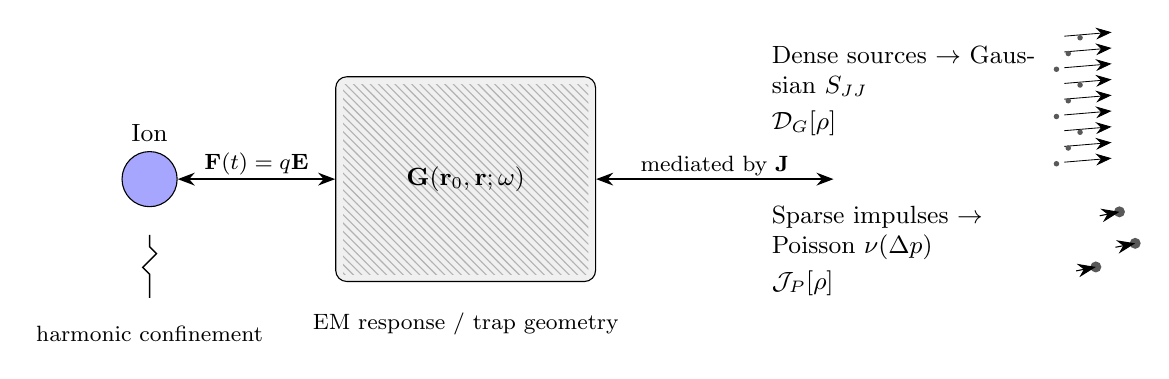
\begin{tikzpicture}[x=1cm,y=1cm,>=Stealth, node distance=2.cm]
  \small
  \tikzset{
    ion/.style={circle, minimum size=7mm, inner sep=0pt, draw=black, fill=blue!35},
    block/.style={draw, rounded corners, fill=gray!12, inner sep=6pt},
    annot/.style={align=left, text width=3.4cm},
    mathnote/.style={font=\footnotesize, inner sep=1pt}
  }
  \node[ion,label=above:{Ion}] (ion) {};
  \draw[line width=0.5pt] ([yshift=-0.35cm]ion.south) -- ++(0,-0.15)
    decorate[decoration=zigzag]{ -- ++(0,-0.5) } -- ++(0,-0.15);
  \node[below=1.4cm of ion, font=\footnotesize] {harmonic confinement};
  \node[block, minimum width=3.3cm, minimum height=2.6cm, right=of ion] (G) {};
  \begin{scope}
    \clip (G.south west) rectangle (G.north east);
    \fill[pattern=north west lines, pattern color=gray!60]
      ($(G.south west)+(0.1,0.1)$) rectangle ($(G.north east)+(-0.1,-0.1)$);
  \end{scope}
  \node at (G) {$\mathbf{G}(\mathbf{r}_0,\mathbf{r};\omega)$};
  \node[mathnote, below=0.35cm of G] {EM response / trap geometry};
  \node[right=of G] (src) {};
  \node[annot, above=1.0 cm of src, anchor=west] (denseLab) {Dense sources $\rightarrow$ Gaussian $S_{JJ}$\\[2pt] $\mathcal{D}_G[\rho]$};
  \foreach \i in {0,...,8}{
    \draw[-{Stealth[length=2mm]}, line width=0.3pt]
      ($(denseLab.east)+(0.2,{-0.9+0.2*\i})$) -- ++(0.6,0.05);
    \fill[black!65] ($(denseLab.east)+({0.1+0.15*mod(\i,3)},{-0.92+0.2*\i})$) circle (0.035);
  }
  \node[annot, below=0.8cm of src, anchor=west] (sparseLab) {Sparse impulses $\rightarrow$ Poisson $\nu(\Delta p)$\\[2pt] $\mathcal{J}_P[\rho]$};
  \foreach \p/\dx in {0.5/0.9, -0.2/0.6, 0.1/1.1}{
    \fill[black!65] ($(sparseLab.east)+(\dx,\p)$) circle (0.07);
    \draw[-{Stealth[length=2.3mm]}] ($(sparseLab.east)+(\dx-0.25,\p-0.05)$) -- ++(0.25,0.05);
  }
  \draw[<->, line width=0.7pt] (ion) -- node[above, mathnote] {$\mathbf{F}(t)=q\mathbf{E}$} (G.west);
  \draw[<->, line width=0.7pt] (G.east) -- node[above, mathnote] {mediated by $\mathbf{J}$} ($(src)+(0.9,0)$);
\end{tikzpicture}

  \caption{\textbf{Universal electromagnetic mediation, distinct source statistics.}
  All motional decoherence mechanisms couple through the same Green tensor $\mathbf{G}(\mathbf{r}_0,\mathbf{r};\omega)$ acting on stochastic environmental currents $\mathbf{J}(\mathbf{r},t)$. 
  The observable dynamics—Gaussian diffusion $\mathcal{D}_G$ versus compound-Poisson jumps $\mathcal{J}_P$—are determined solely by the statistics of $\mathbf{J}$: dense sources produce Gaussian correlations $S_{JJ}$, while sparse events yield a L\'evy measure $\nu(\Delta p)$ over momentum kicks. For Gaussian noise, heating and dephasing are independent channels controlled by different spectral regions; for impulsive noise, each kick induces both energy change and phase shift.}
  \label{fig:em_mediation}
\end{figure}

\paragraph{Theoretical foundation.}
The three categories arise naturally from established open-quantum-systems theory. Field-induced diffusion follows from the fluctuation-dissipation relation in macroscopic QED, where $S_E(\omega)$ is determined by $\mathbf{G}$ and material response~\cite{ScheelBuhmann2008,BrownnuttRMP2015,BuhmannDispersionForcesII}. Collision-induced jumps emerge from the quantum linear Boltzmann equation~\cite{HornbergerSipe2003,VacchiniHornberger2009,OghittuNJPhys2023}. Both are special cases of the L\'evy--Khintchine decomposition for translation-covariant quantum Markov semigroups~\cite{Holevo1993,VacchiniJMathPhys2001}, whose sum is rigorously justified under weak coupling and Markov approximations~\cite{BreuerPetruccione2002}. 

Our contribution is not to re-derive these results but to synthesize them into a unified experimental framework: we connect microscopic mechanisms (scattering cross-sections, current correlations) to observable signatures of motional decoherence—including both energy and phase dynamics—through explicit, measurable discriminants.

\paragraph{Predictive guidance for experiments.}
The categorization yields concrete experimental design principles. A key insight is the separation of concerns: \emph{temporal statistics} (characterized by the dimensionless parameter $\lambda\tau$, the product of event rate and interrogation time) determine which observables are informative, while \emph{spectral content} determines the relative weight of heating versus dephasing within each category.

For temporal statistics, $\lambda\tau$ determines measurement strategy:
\begin{itemize}[leftmargin=*,nosep]
\item $\lambda\tau \gg 1$ (diffusive regime): Use spectral methods—heating rates $\dot{n} \propto S_F(\omega_t)$, dephasing times from low-frequency spectrum $S_{\delta\omega}(\Omega)$, sideband asymmetry scans, and field correlation measurements. Heating and dephasing are independent channels.

\item $\lambda\tau \sim 1$ (intermediate regime): Measure higher-order cumulants (skewness $\kappa_3$, kurtosis $\kappa_4$) and Allan variance rollover near $\tau \sim 1/\lambda$ to detect non-Gaussian contributions. Energy and phase statistics become correlated.

\item $\lambda\tau \ll 1$ (jump-resolved regime): Record waiting-time distributions (exponential for Poisson, power-law for L\'evy) and jump-size histograms $P(\Delta n)$ directly related to $\nu(\Delta p)$. Each event produces both energy jump and phase reset.
\end{itemize}

Crucially, $\lambda\tau$ characterizes \emph{event statistics}, not spectral content. A Gaussian noise source with 1/f spectrum ($\lambda\tau \gg 1$) can produce strong dephasing but weak heating; conversely, a Poisson collision process ($\lambda\tau \ll 1$) with large momentum transfer produces primarily heating. The framework accounts for both aspects independently.

Table~\ref{tab:discriminants} provides the complete decision map with required shot counts and statistical power estimates. Section~\ref{sec:inference_protocol} details stroboscopic measurement protocols, while Sec.~\ref{sec:scattering_models} connects specific scattering mechanisms (Langevin, hard-sphere, charge exchange) to predicted observables.

\paragraph{Scope and limitations.}
The framework assumes: (i)~harmonic confinement with linear coupling $H_{\text{int}} = -qxE_x$, valid when ion motion remains small compared to field-variation scales; (ii)~Markovian bath dynamics, requiring environmental correlation times short compared to trap period $\omega_t^{-1}$; (iii)~stationary noise statistics. For weakly anharmonic traps, position-dependent frequency shifts $\delta\omega(t) \propto \beta \delta x(t)$ or $\gamma (\delta x(t))^2$ can enhance dephasing even when field noise itself is weak. Extensions to non-Markovian memory kernels and multi-ion correlated dynamics are discussed but not fully developed. Within these approximations, the categorization is exhaustive for single-ion motional decoherence.
Although the L\'evy--Khintchine structure is universal across open quantum systems, here we restrict attention to trapped-ion motion, where control and observables allow us to cleanly contrast Gaussian and jump-dominated noise in practice.
%==================================================
%  Section 2: Noise Regimes and Motional Responses
%==================================================
\section{Noise Regimes and Motional Responses}
\label{sec:noise_regimes}

Environmental fluctuations couple to a trapped ion’s harmonic motion either
as effectively continuous fields or as discrete impulses.  Both arise from
stochastic current sources $J(\mathbf r,t)$ and are mediated by the trap’s
electromagnetic Green tensor $G(\mathbf r_0,\mathbf r;\omega)$.

In the following, we use the term \emph{motional decoherence} to refer
collectively to all processes by which environmental noise degrades the
purity of the ion’s motional state. This encompasses both \emph{heating}—
energy exchange via resonant force fluctuations—and \emph{dephasing}—
phase diffusion caused by slow potential variations. Where the distinction
matters for understanding spectral origins or experimental signatures,
we refer to heating and dephasing explicitly.

To classify temporal statistics we use the dimensionless product
$\lambda\tau$, which counts independent events within one experimental
interrogation time~$\tau$.  For impulsive processes $\lambda$ denotes the
Poisson rate of discrete events; for continuous Gaussian fields,
$\lambda^{-1}$ represents an effective correlation time $\tau_c$, so that
$\lambda\tau\!\sim\!\tau/\tau_c$ measures the number of independent
fluctuation intervals.  \emph{Crucially, $\lambda\tau$ characterizes event
statistics, not the frequency content of the noise spectrum.}
Heating and dephasing depend on \emph{spectral weight} at different
frequencies, independent of whether the statistics are diffusive or sparse.

%----------------------------------------
\paragraph{Diffusive regime ($\lambda\tau\!\gg\!1$).}
Many independent fluctuations accumulate and the central-limit theorem
applies: force statistics are well described by a Gaussian process.
The ion’s energy changes at a rate set by the near-resonant spectral weight
of the force noise filtered by the mechanical susceptibility
$\chi(\omega)$ (derived in Sec.~\ref{sec:theory_foundations}):
\[
\frac{d\langle n\rangle}{dt}
 = \frac{1}{4 m \hbar \omega_t}\!\int_{-\infty}^{\infty}\!
   |\chi(\omega)|^{2} S_F(\omega)\,d\omega,
\qquad S_F(\omega)=q^{2}S_E(\omega).
\]
The process is statistically Gaussian, but this says nothing about phase
coherence: dephasing can be strong if low-frequency spectral weight is large
(e.g.\ $1/f$ noise), and weak if such weight is small.

%----------------------------------------
\paragraph{Intermediate regime ($\lambda\tau\!\sim\!1$).}
Only a few fluctuations occur within~$\tau$.  The motion alternates between
free evolution and discrete perturbations, producing non-Gaussian
statistics with measurable higher-order cumulants and characteristic
roll-overs in the Allan variance.  Each impulse contributes \emph{both}
energy change and a phase shift, so motional decoherence manifests through
coupled energy and phase fluctuations.
This regime is particularly diagnostic of underlying source statistics
(cf.\ Sec.~\ref{sec:discriminants_summary}).

%----------------------------------------
\paragraph{Sparse regime ($\lambda\tau\!\ll\!1$).}
Isolated impulses are resolvable in time with exponential waiting-time
distribution $p(t)=\lambda e^{-\lambda t}$.  Between impulses the oscillator
evolves coherently; each rare impulse applies a finite displacement in
phase space, producing a discrete energy jump together with a phase reset.
The observables are step-like heating and discrete, resolvable phase
discontinuities.

%----------------------------------------
\subsection*{Heating and Dephasing Channels: Spectral View and Operators}

Environmental noise modifies (i) the \emph{energy} of the oscillator
(heating) and (ii) the \emph{phase} of its coherent motion (dephasing).
These effects are controlled by different parts of the spectrum of the
electric field at the ion.

\begin{itemize}
  \item \textbf{Heating (energy exchange).}
  With $H_\mathrm{int}=-q x E(t)$, the heating rate is determined by the
  force-noise spectrum $S_F(\omega)=q^2 S_E(\omega)$ filtered by the
  mechanical susceptibility $|\chi(\omega)|^{2}$.  In the high-$Q$ limit the
  integral above reduces to the familiar near-resonant expression
  $\dot{\langle n\rangle}\!\approx\! (q^{2}/4m\hbar\omega_t)\,S_E(\omega_t)$.
  Off-resonant spectral weight contributes according to
  $|\chi(\omega)|^{2}$ and should not be neglected when linewidths are broad
  or spectra structured.

  \item \textbf{Dephasing (phase diffusion without energy exchange).}
  Slow fluctuations of the trapping potential or stray fields modulate the
  instantaneous frequency
  $\omega_t\!\rightarrow\!\omega_t+\delta\omega(t)$,
  producing a random phase
  $\phi(t)=\int_{0}^{t}\delta\omega(t')\,dt'.$
  The coherence of a motional superposition decays as
  $\exp[-\tfrac{1}{2}\langle(\Delta\phi)^{2}\rangle]$, with
  \[
    \langle(\Delta\phi)^{2}\rangle
      = 2\!\int_{0}^{\infty}\! S_{\delta\omega}(\Omega)
        \!\left(\frac{\sin(\Omega t/2)}{\Omega/2}\right)^{2}\! d\Omega .
  \]
  In realistic traps, however, the potential includes higher-order terms
  beyond the harmonic approximation,
  \[
    U(x) = \tfrac{1}{2}m\omega_t^2x^2 + \beta x^3 + \gamma x^4 + \dots .
  \]
  While the master equation derived in Sec.~\ref{sec:theory_foundations}
  assumes harmonic confinement and linear coupling, anharmonic corrections
  to dephasing rates can be incorporated perturbatively when
  $|\beta|x_0 \ll m\omega_t^2$ and $|\gamma|x_0^2 \ll m\omega_t^2$.
  In this weakly anharmonic regime, small shifts of the equilibrium position
  caused by $\delta E(t)$ change the local curvature experienced by the ion
  and thus the instantaneous secular frequency.
  For cubic terms the frequency shift scales linearly with displacement,
  $\delta\omega(t) \propto \beta\,\delta x(t)$,
  whereas quartic terms contribute quadratically,
  $\delta\omega(t) \propto \gamma\,(\delta x(t))^{2}$.
  These position-dependent curvature changes can substantially enhance
  motional dephasing even when the field noise itself is weak.
  True frequency noise also arises from electric-field gradients or
  parametric variations of the RF or control voltages that modulate the
  confining curvature.  In such cases the spectrum
  $S_{\delta\omega}(\Omega)$ is directly linked to the low-frequency
  component of the field-gradient or control-voltage noise spectrum.
  In the Markov limit $S_{\delta\omega}(0)$ defines an exponential
  dephasing time~$T_{\phi}$, while quasi-static variations produce Gaussian
  temporal decay.
\end{itemize}

\noindent\textbf{Unified impulse picture.}
A single momentum impulse implements the unitary displacement
$U_{\Delta p}=\exp[-i\,\Delta p\,x/\hbar]$,
which simultaneously increases energy and shifts the phase of the coherent
state.  Accordingly, it is incorrect to assign ``kicks~$\rightarrow$~heating''
and ``timing~$\rightarrow$~dephasing'' to separate channels; both arise from
the same operator action, while their \emph{observed balance} is governed by
the spectral content of $S_E(\omega)$ and the trap’s susceptibility.

\medskip
\noindent\textbf{Summary.}
The parameter $\lambda\tau$ organizes temporal statistics
(diffusive~$\leftrightarrow$~sparse), whereas heating and dephasing are set by
\emph{which} parts of the spectrum carry power:
near~$\omega_t$ for heating and near~0 for dephasing.
Either contribution can dominate in any regime.

\section{Theoretical Framework: From Keldysh to L\'evy}
\label{sec:theory_foundations}

\subsection{System--Bath Setup}
We model a single trapped ion of charge $q$ and mass $m$, confined harmonically at frequency $\omega_t$ along $x$.
The ion couples to the fluctuating electric field $\mathbf{E}(\mathbf{r}_0,t)$ at its equilibrium position $\mathbf{r}_0$, generated by stochastic currents $\mathbf{J}(\mathbf{r},t)$ in the environment.
The Hamiltonian is
\begin{equation}
H = \frac{p^2}{2m} + \tfrac{1}{2} m \omega_t^2 x^2 - q x E_x(\mathbf{r}_0,t).
\end{equation}
The field obeys Maxwell's equations with sources $\mathbf{J}$, and the ion couples linearly via $H_{\text{int}} = -q x E_x$.

\subsection{Electromagnetic Green Tensor}
The electric field is expressed through the dyadic Green tensor $\mathbf{G}$ relating currents to fields in frequency space,
\begin{equation}
\mathbf{E}(\mathbf{r}_0,\omega) = \mathrm{i}\mu_0 \omega \int d^3r\, \mathbf{G}(\mathbf{r}_0,\mathbf{r};\omega) \mathbf{J}(\mathbf{r},\omega).
\end{equation}
Here $\mathbf{G}$ satisfies the Helmholtz equation
\begin{equation}
\left[\nabla\times\nabla\times - \frac{\omega^2}{c^2}\varepsilon(\mathbf{r},\omega)\right]\mathbf{G}(\mathbf{r},\mathbf{r}';\omega) = \delta(\mathbf{r}-\mathbf{r}')\mathbf{I}.
\end{equation}
The permittivity $\varepsilon(\mathbf{r},\omega)$ encodes electrode/dielectric response; in practice $\mathbf{G}$ is computed numerically for trap geometry.

\subsection{Keldysh Formalism}
The ion+EM+bath system is described by a Keldysh action~\cite{Kamenev2011}, doubling fields on forward/backward contours.
Integrating out EM modes yields an effective action for the ion with force-force correlator
\begin{equation}
S_F(\omega) = q^2 \int d^3r d^3r'\, G_{x\alpha}(\mathbf{r}_0,\mathbf{r};\omega)\, S_{JJ}^{\alpha\beta}(\mathbf{r},\mathbf{r}';\omega)\, G^*_{x\beta}(\mathbf{r}_0,\mathbf{r}';\omega).
\label{eq:SF}
\end{equation}
\textit{Key result:} all environmental noise enters via $S_F(\omega)$, the current spectrum $S_{JJ}$ filtered by trap response $|\mathbf{G}(\omega)|^2$.

\subsection{Gaussian Bath $\to$ Diffusion}
For dense, weakly coupled baths, $\mathbf{J}$ is Gaussian with correlations $S_{JJ}$.
The effective master equation is of Lindblad form
\begin{equation}
\dot{\rho} = -\mathrm{i}[H_0,\rho] + \Gamma_\uparrow \mathcal{D}[a^\dagger]\rho + \Gamma_\downarrow \mathcal{D}[a]\rho,
\end{equation}
with rates $\Gamma_{\uparrow,\downarrow} \propto S_F(\pm\omega_t)$.
The heating rate is
\begin{equation}
\Gamma_{\text{heat}} = \Gamma_\uparrow - \Gamma_\downarrow = \frac{x_0^2}{\hbar^2}\left[S_F(+\omega_t) - S_F(-\omega_t)\right],
\end{equation}
with $x_0=\sqrt{\hbar/(2m\omega_t)}$.
In equilibrium, detailed balance gives $S_F(-\omega_t)/S_F(+\omega_t)=e^{-\hbar\omega_t/k_BT}$.

\subsection{Poisson Bath $\to$ Jumps}
For sparse scatterers, $\mathbf{J}$ is a sum of impulses $\mathbf{j}_k(t-t_k)$.
The effective dynamics are compound-Poisson: each event imparts momentum $\Delta p$, with rate $\lambda$ and distribution $\nu(\Delta p)$.
The generator is
\begin{equation}
\mathcal{J}_P\rho = \lambda \int d(\Delta p)\, \nu(\Delta p)\,\left[e^{-\mathrm{i}\Delta p x/\hbar}\rho e^{+\mathrm{i}\Delta p x/\hbar}-\rho\right].
\end{equation}

\subsection{Unified L\'evy--Khintchine Form}
The full ion master equation is thus
\begin{equation}
\dot{\rho} = -\mathrm{i}[H_0,\rho] + \mathcal{D}_G[\rho] + \mathcal{J}_P[\rho],
\label{eq:levy-box}
\end{equation}
a L\'evy--Khintchine generator: Gaussian diffusion $\mathcal{D}_G$ plus compound-Poisson jumps $\mathcal{J}_P$.

\paragraph{Crossover regimes and dominance criteria.}
The relative importance of diffusion versus jumps is set by dimensionless ratios:
\begin{equation}
\frac{\text{jump heating}}{\text{Gaussian heating}}
\sim \frac{\lambda \langle (\Delta p)^2 \rangle}{x_0^2 S_F(\omega_t)/\hbar^2},
\quad
\frac{\text{events per measurement}}{\text{one}}
\sim \lambda \tau.
\end{equation}
Three regimes emerge naturally:
\begin{itemize}
\item \textbf{Diffusive limit} ($\lambda \tau \gg 1$, small $\langle(\Delta p)^2\rangle$):
  Jumps coalesce into effective Gaussian noise;
  $\kappa_3, \kappa_4 \to 0$;
  Allan variance $\sigma_A^2(\tau) \propto \tau^{-1}$.
\item \textbf{Intermediate regime} ($\lambda \tau \sim 1{-}10$):
  Both terms in Eq.~\eqref{eq:levy-box} contribute comparably;
  non-Gaussian cumulants measurable ($\kappa_3/\kappa_2^{3/2} \sim 0.3{-}1$);
  Allan variance shows rollover near $\tau \sim 1/\lambda$
  (Table~\ref{tab:discriminants}, Sec.~\ref{sec:discriminants_summary}).
\item \textbf{Poisson limit} ($\lambda \tau \ll 1$, large $\langle(\Delta p)^2\rangle$):
  Discrete, resolvable jumps dominate;
  waiting-time statistics exponential;
  $P(\Delta n)$ determined by $\nu(\Delta n)$ directly.
\end{itemize}
Experimentally, the intermediate regime is often the most informative:
it separates mechanisms via higher-order statistics while still accumulating
measurable events on laboratory timescales.
Table~\ref{tab:discriminants} provides experimentally accessible discriminants optimized for this intermediate regime, where neither limit dominates and model selection becomes nontrivial.

\subsection{From Momentum to Phonon Jumps}
Experimentally, jumps are resolved in motional phonon number $n$.
Momentum transfer $\Delta p$ maps to phonon transitions via
\begin{equation}
\nu(\Delta n) = \int d(\Delta p)\,\nu(\Delta p)\,\sum_{n'} P_{n\to n'}(\Delta p)\, \delta(\Delta n-(n'-n)),
\label{eq:nu_to_deltan}
\end{equation}
with $P_{n\to n'}(\Delta p)=|\langle n'|e^{-\mathrm{i}\Delta p x/\hbar}|n\rangle|^2$.
This connects scattering cross-sections $d\sigma/d\Omega$ to measurable $\nu(\Delta n)$ (see Sec.~\ref{sec:scattering-models}).

\paragraph{Takeaway.}
The ion's heating is universally described by Eq.~\eqref{eq:levy-box}, independent of microscopic mechanism.
The experimentally accessible regime is often \emph{intermediate}, where $\lambda \tau \sim 1{-}10$ and both Gaussian and jump terms contribute measurably.
Section~\ref{sec:observable_signatures} develops observables—cumulants, waiting times, and Allan variance—that discriminate $\mathcal{D}_G$ versus $\mathcal{J}_P$ even when both are present simultaneously.

\subsection{Heavy-Tailed L\'evy Processes}
Heavy-tailed L\'evy flights extend the compound-Poisson picture to jump-size distributions with divergent variance,
$\nu(\Delta p)\!\propto\! |\Delta p|^{-1-\alpha}$ for $0<\alpha<2$.
In this regime the second moment diverges and the central-limit theorem no longer applies, producing anomalous diffusion $\langle (\Delta x)^2 \rangle \propto t^{2/\alpha}$.
Such processes may arise from rare large-impulse events—e.g. Coulomb scattering on charged dust grains or micro-discharge spikes.
Their generator replaces the finite-variance term in Eq.~(7) by the fractional Laplacian $-D_\alpha(-\partial_x^2)^{\alpha/2}$.
A full quantitative treatment is left for future work.

The heavy-tailed form $\nu(\Delta p)\!\propto\!|\Delta p|^{-1-\alpha}$ with
$0<\alpha<2$ implies a corresponding power-law distribution of phonon jumps
via Eq.~\eqref{eq:nu_to_deltan},
$P(\Delta n)\!\propto\!|\Delta n|^{-1-\alpha}$.
Because the variance of $\nu(\Delta p)$ diverges for $\alpha<2$, the
central-limit theorem no longer applies and the resulting motion follows a
fractional diffusion process.
In the time domain, the mean-square displacement scales anomalously as
$\langle(\Delta x)^2\rangle\!\propto\!t^{2/\alpha}$, producing an Allan
variance with slope $\,\sigma^2_A(\tau)\!\propto\!\tau^{-(2/\alpha-1)}$.
This anomalous exponent yields the non-integer slopes and long tails listed
for heavy-tailed L\'evy processes in Table~\ref{tab:discriminants}.
A detailed quantitative treatment of fractional diffusion dynamics will be
presented in future work.

\section{Observable Signatures and Scattering Models}
\label{sec:scattering-models}
\label{sec:observable_signatures}
The unified L\'evy--Khintchine generator (Eq.~\ref{eq:levy-box}) predicts that ion heating arises from a combination of Gaussian diffusion and compound-Poisson jumps.
We develop experimentally distinguishable signatures that allow independent extraction of these components.

\noindent\textbf{(a) Langevin induced-dipole scattering}\quad
\emph{Regime:} Low-energy ion--neutral collisions with polarizable neutral ($E \lesssim 1$~eV).\\
\emph{Cross-section:}
\[
\frac{d\sigma}{d\Omega} =
\frac{\alpha e^2}{8\pi\epsilon_0^2 \mu^2 v^4}\,
\frac{\sin^2\theta}{(1-\cos\theta)^4},
\]
with $\alpha$ the neutral polarizability.
The total Langevin cross-section is $\sigma_{\rm L} = \pi e\sqrt{\alpha/(\epsilon_0 E)} \propto E^{-1/2}$.\\
\emph{Key feature:} Soft divergence at small $\Delta p$ (forward scattering), cut off by quantum diffraction $b_{\min}\sim \hbar/\mu v$.\\
\emph{Consequence:} $\nu(\Delta p)$ has enhanced small-$\Delta p$ weight; CLT $\to$ near-Gaussian heating but with fat tails.\\
\emph{Relevant systems:} Ca$^+$, Sr$^+$, Ba$^+$ with H$_2$, N$_2$, Ar backgrounds.

\textit{Universal behavior:}
The Langevin form is \emph{universal} in that it depends only on the neutral's polarizability $\alpha$, not on molecular details.
This implies that $\nu(\Delta p)$ is parametrized by just $\alpha$ and the velocity distribution $f(v)$, reducing the inference problem to fitting $\lambda$ (or equivalently $n_g$) and $T$ from experimental data.
Departures from universality—resonant charge exchange, short-range chemistry, or high-energy collisions—introduce additional structure in $\nu(\Delta p)$ and require species-specific cross-sections.

\medskip
\noindent\textbf{(b) Hard-sphere scattering}\quad
\emph{Regime:} Classical collisions with effective radius $R$.\\
\emph{Cross-section:}
\[
\frac{d\sigma}{d\Omega} = \frac{R^2}{4\pi}.
\]
\emph{Key feature:} Isotropic scattering, momentum transfer peaked at $|\Delta p|=2\mu v$.\\
\emph{Consequence:} $\nu(\Delta p)$ becomes sharply peaked, yielding bimodal $P(\Delta n)$.\\
\emph{Relevant systems:} Test gases (He, Ne) in controlled background studies.

\medskip
\noindent\textbf{(c) Resonant charge exchange}\quad
\emph{Regime:} Ion--atom collisions with same species (e.g., Ca$^+$ + Ca).\\
\emph{Cross-section:}
\[
\sigma_{\rm CX}(E) \approx \sigma_0\left(1 + \frac{E}{E_0}\right)^{-1/2},
\]
with $\sigma_0$ set by resonant channel strength.
Charge exchange swaps internal states, producing state-dependent heating.

\medskip
\noindent\textbf{(d) Charged dust grains}\quad
\emph{Regime:} Occasional Coulomb interactions with micron-scale charged particles.\\
\emph{Characteristic:} Large impulse events with $|\Delta p| \gg \mu v$, leading to heavy-tailed $\nu(\Delta p)$.
\emph{Observable:} Rare, multi-phonon jumps and long-lived charge-induced fields.

These models feed directly into the inference protocol of Sec.~\ref{sec:inference-protocol} and the discriminants summarized in Sec.~\ref{sec:discriminants-table}.

\section{Electromagnetic Mediation Pathways}
Electromagnetic interactions mediate every noise source to the trapped ion.
Starting from stochastic current sources $\mathbf{J}(\mathbf{r},t)$, the electric field at the ion position is filtered by the dyadic Green tensor $\mathbf{G}(\mathbf{r}_0,\mathbf{r};\omega)$:
\begin{equation}
\mathbf{E}(\mathbf{r}_0,\omega) = \mathrm{i}\mu_0\omega \int d^3 r\, \mathbf{G}(\mathbf{r}_0,\mathbf{r};\omega) \mathbf{J}(\mathbf{r},\omega).
\end{equation}
Regardless of the microscopic origin of $\mathbf{J}$, the force spectrum $S_F(\omega)$ entering the master equation is
\begin{equation}
S_F(\omega) = q^2 \int d^3 r d^3 r'\, G_{x\alpha}(\mathbf{r}_0,\mathbf{r};\omega) S_{JJ}^{\alpha\beta}(\mathbf{r},\mathbf{r}';\omega) G^{*}_{x\beta}(\mathbf{r}_0,\mathbf{r}';\omega).
\end{equation}

\paragraph{Practical modeling.}
Trap geometries are encoded via $\mathbf{G}$, typically computed with boundary-element or finite-element solvers.
Once tabulated, $\mathbf{G}$ enables rapid evaluation of candidate noise sources:
\begin{itemize}
  \item \textbf{Technical fields:} Johnson noise or control electrode pickup yields Gaussian $S_{JJ}$.
  \item \textbf{Gas collisions:} Charged or neutral scatterers contribute impulses parameterized by cross-sections (Sec.~\ref{sec:scattering-models}).
  \item \textbf{Surface dipoles:} Patch potentials manifest as correlated dipole moments with colored spectra.
\end{itemize}

\paragraph{Connection to figures.}
Figure~\ref{fig:em_mediation} visualizes the mediation network, while spatial coherence effects for extended trajectories are shown in Fig.~\ref{fig:trajectory_coherence}.

%==================================================
%  Section 6: Model Assumptions and Validity Domain
%==================================================
\section{Model Assumptions and Validity Domain}
\label{sec:model_assumptions}

The unified L\'evy--Keldysh framework presented in the preceding sections relies on several
physical and mathematical approximations that define its domain of validity.
We summarize these explicitly below to delineate the scope of applicability
and to prevent over-interpretation beyond their justified range.

\subsection{Linear Coupling Approximation}
The system--bath interaction Hamiltonian is taken to be
\begin{equation}
H_\mathrm{int}(t) = -q\,x(t)\,E_x(r_0,t),
\end{equation}
which assumes a linear coupling between the ion's displacement and the local electric field.
This approximation is accurate when the ion's motion remains small compared to the spatial
scale over which the field varies, \(x \ll r_0\).  
In regimes with strong anharmonic confinement or large motional excitation,
higher-order coupling terms \(x^2 E'(r_0,t)\) may contribute and modify the effective noise spectrum.

\subsection{Markovian Bath Assumption}
The derivation of the L\'evy--Khintchine generator presumes a memoryless environment,
where the bath correlation time \(\tau_c\) is short compared to the ion's motional period
\(\omega_t^{-1}\).  
Under this condition, the noise statistics can be encoded in a time-independent generator.
For slow environmental processes such as \(1/f\) charge-patch fluctuations,
a non-Markovian generalization with an explicit memory kernel \(K(t-t')\)
would be required to accurately capture temporal correlations.

\subsection{Stationarity and Ergodicity}
The framework assumes stationary noise statistics,
i.e.\ correlation functions depend only on time differences.
Ergodicity ensures that ensemble averages coincide with long-time averages,
enabling experimental inference from single-trajectory measurements.

\subsection{Trap Geometry and Green Tensor}
All spatial field correlations are expressed through the electromagnetic Green tensor
\(G(r,r';\omega)\), which is geometry-dependent and, in practice,
evaluated numerically for a given electrode configuration.
Uncertainties in geometry modeling directly propagate into predictions
of heating rates and noise spectra.  
Validation of \(G\) against experimental benchmarks is therefore essential
for quantitative accuracy.

\subsection{Summary of Validity Domain}
The present formalism accurately describes single-ion motional heating
in the linear, Markovian, and stationary limits.
Extensions to multi-ion or correlated environments are conceptually straightforward
but lie beyond the current manuscript's scope and will be pursued in future work.

\section{Spatial and Temporal Coherence Effects}
\label{sec:spatial-coherence}
\begin{tcolorbox}[title=Fast scatterers: spatial coherence effects]
For a moving scatterer with trajectory $\mathbf{r}_k(t)=\mathbf{r}_0+\mathbf{v}t$, the current density is
\[
\mathbf{j}_k(\mathbf{r},t) = \mathbf{j}^{(0)}_k(t)\,\delta^{(3)}(\mathbf{r}-\mathbf{r}_k(t)).
\]
The force spectrum becomes
\[
F_k(\omega) = q \int dt\, e^{\mathrm{i}\omega t}\,\mathbf{G}(\mathbf{r}_0,\mathbf{r}_k(t);\omega)\cdot\mathbf{j}^{(0)}_k(t).
\]

\textbf{Velocity regimes:}
\begin{itemize}\itemsep0.2em
  \item Thermal background ($v \sim 500$~m/s, $\tau_{\rm coll}\sim 10$~ps): $v\tau_{\rm coll}\sim 5$~nm $\ll L_{\rm trap}$ $\to$ point-impulse limit.
  \item Fast cosmics ($v\sim 0.1c$, $\tau_{\rm coll}\sim 1$~ps): $v\tau_{\rm coll}\sim 30~\mu$m $\sim L_{\rm trap}$ $\to$ extended-coherence regime.
\end{itemize}

\textbf{Impact:} Spatial variation of $\mathbf{G}$ introduces directional coupling, $|F_k(\omega)|^2 \propto |\hat{\mathbf{v}}\cdot\nabla\mathbf{G}|^2$, breaking isotropy.

\textbf{Observable:} Anisotropic heating as a function of trap orientation relative to a collimated beam or fast flux (see Fig.~\ref{fig:trajectory_coherence}).
\end{tcolorbox}

\begin{figure}[t]
  \centering
  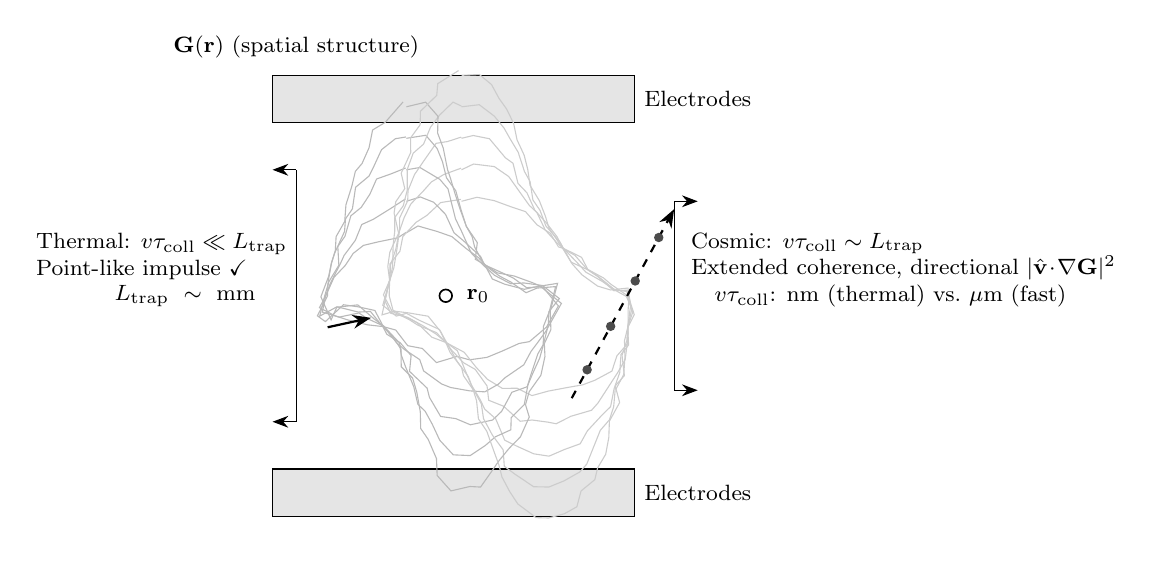
\begin{tikzpicture}[x=1cm,y=1cm,>=Stealth]
  \small
  \def\W{4.6}
  \def\H{6.2}
  \def\gap{3.2}
  \node at (0,0) {};
  \draw[fill=gray!20] (-1.5,  \gap/2+0.6) rectangle (\W-1.5,  \gap/2+1.2);
  \draw[fill=gray!20] (-1.5, -\gap/2-1.2) rectangle (\W-1.5, -\gap/2-0.6);
  \node[font=\footnotesize] at (\W-1.5+0.8,  \gap/2+0.9) {Electrodes};
  \node[font=\footnotesize] at (\W-1.5+0.8, -\gap/2-0.9) {Electrodes};
  \begin{scope}
    \clip (-1.5, -\H/2) rectangle (\W-1.5, \H/2);
    \foreach \a in {0.8,1.2,1.6,2.0,2.4}{
      \draw[gray!55, decorate, decoration={random steps, segment length=2mm, amplitude=0.6mm}]
        plot[smooth cycle, tension=1] coordinates{
          (-0.8,0) (0.2,\a) (1.2,0.4) (2.0,-0.2) (1.0,-\a) (-0.1,-0.4)};
      \draw[gray!40, decorate, decoration={random steps, segment length=2mm, amplitude=0.5mm}]
        plot[smooth cycle, tension=1] coordinates{
          (0.0,0.2) (0.9,\a+0.4) (2.2,0.6) (3.0,-0.4) (2.0,-\a-0.4) (0.7,-0.6)};
    }
  \end{scope}
  \node[font=\footnotesize, anchor=south] at (-1.2, \H/2-0.2) {$\mathbf{G}(\mathbf{r})$ (spatial structure)};
  \filldraw[fill=white, draw=black, line width=0.6pt] (0.7,0) circle (0.08);
  \node[font=\footnotesize, anchor=west] at (0.85,0) {$\mathbf{r}_0$};
  \draw[thick, -Stealth] (-0.8, -0.4) -- ++(0.55,0.12);
  \node[font=\footnotesize, align=left, anchor=east] at (-1.2,0.5)
    {Thermal: $v\tau_{\rm coll} \ll L_{\rm trap}$\\Point-like impulse \checkmark};
  \draw[thick, dashed, -Stealth] (2.3, -1.3) -- (3.6, 1.1);
  \foreach \t in {0.15,0.38,0.62,0.85}{
    \fill[black!70] ($(2.3, -1.3)!{\t}!(3.6,1.1)$) circle (0.06);
  }
  \node[font=\footnotesize, align=left, anchor=west] at (3.7, 0.5)
    {Cosmic: $v\tau_{\rm coll} \sim L_{\rm trap}$\\Extended coherence, directional $|\hat{\mathbf{v}}\!\cdot\!\nabla\mathbf{G}|^2$};
  \draw[very thin] (-1.2,-\gap/2) -- (-1.2,\gap/2);
  \draw[-{Stealth[length=2mm]}] (-1.2,\gap/2) -- ++(-0.3,0);
  \draw[-{Stealth[length=2mm]}] (-1.2,-\gap/2) -- ++(-0.3,0);
  \node[font=\footnotesize, align=center, anchor=east] at (-1.6,0) {$L_{\rm trap}\ \sim\ \mathrm{mm}$};
  \draw[very thin] (\W-1.0,-1.2) -- (\W-1.0,1.2);
  \draw[-{Stealth[length=2mm]}] (\W-1.0,1.2) -- ++(0.3,0);
  \draw[-{Stealth[length=2mm]}] (\W-1.0,-1.2) -- ++(0.3,0);
  \node[font=\footnotesize, align=center, anchor=west] at (\W-0.6,0)
    {$v\tau_{\rm coll}$: nm (thermal) vs.\ $\mu$m (fast)};
\end{tikzpicture}

  \caption{Representative geometry for extended trajectories producing anisotropic heating signatures.
  The path length $v\tau_{\rm coll}$ relative to trap dimensions $L_{\rm trap}$ determines whether the point-impulse approximation holds.}
  \label{fig:trajectory_coherence}
\end{figure}

\section{Inference Protocol}
\label{sec:inference-protocol}
\label{sec:inference_protocol}
\paragraph{Recommended stroboscopic sequence.}
\begin{enumerate}\itemsep0.2em
  \item Prepare motional ground state $\lvert n=0\rangle$ (or a calibrated thermal $\langle n\rangle$).
  \item Wait time $\tau$ (free evolution under noise).
  \item Read out $n$ via sideband thermometry or fluorescence.
  \item Repeat $N$ times $\Rightarrow$ histogram $P(n\,|\,\tau)$ and time series $n(t)$.
\end{enumerate}

\begin{table}[h]
  \centering
  \renewcommand{\arraystretch}{1.15}
  \begin{tabularx}{0.9\textwidth}{>{\raggedright\arraybackslash}X>{\raggedleft\arraybackslash}p{4.2cm}}
    \hline
    \textbf{Target quantity} & \textbf{Required shots/events (order-of-magnitude)} \\
    \hline
    Detect $\kappa_3 \neq 0$ at $3\sigma$ & $\sim 10^4$ stroboscopic shots \\
    Reconstruct $\nu(\Delta n)$ (5 bins)  & $\sim 10^5$ shots \\
    Test heavy-tail exponent $\alpha$      & $\sim 10^6$ events \\
    Allan variance rollover near $1/\lambda$ & hours of continuous trace \\
    Sideband asymmetry vs.\ $\omega$ map   & $\sim 10^2$ frequency scans \\
    \hline
  \end{tabularx}
\end{table}

\subsection{Stroboscopic measurement: detailed protocol}
\paragraph{Definition.}
A \emph{stroboscopic measurement} consists of repeated cycles
\[
  \text{Prepare} \to \text{Wait } \tau \to \text{Readout} \to \text{Reset}
\]
with fixed waiting time $\tau$ and $N$ independent repetitions.
The observable is the phonon number $n$ after free evolution under noise.

\paragraph{Pulse sequence and timing.}
\begin{enumerate}
  \item \textbf{Doppler cooling} ($t_{\rm cool} \sim 1{-}2\,\text{ms}$): Bring the ion near the ground state via red-detuned cooling.
  \item \textbf{Resolved-sideband cooling} ($t_{\rm RSBC} \sim 1$~ms): Achieve $n < 0.1$ by sideband pulses and optical pumping.
  \item \textbf{Idle/noise evolution} ($t=\tau$): Allow environmental noise to act.
  \item \textbf{Readout}: Use blue-sideband ratio or time-of-flight to infer $n$.
  \item \textbf{Reset}: Re-cool before the next cycle.
\end{enumerate}

\paragraph{Bayesian inference.}
Given histograms $P(n\,|\,\tau)$ for multiple waiting times, we infer model parameters $\Theta = \{\lambda, \alpha, S_F(\omega)\}$ via hierarchical Bayesian fits.
Posterior sampling (e.g., Hamiltonian Monte Carlo) yields credible intervals and allows evidence comparisons between models.

\section{Discriminants Summary}
\label{sec:discriminants_summary}
\begin{table}[h]
  \centering
  \renewcommand{\arraystretch}{1.2}
  \begin{tabularx}{\textwidth}{>{\raggedright\arraybackslash}p{3.2cm}
                                    >{\raggedright\arraybackslash}X
                                    >{\raggedright\arraybackslash}X
                                    >{\raggedright\arraybackslash}X
                                    >{\raggedright\arraybackslash}p{2.8cm}}
    \hline
    \textbf{Observable}
    & \textbf{Gaussian bath}
    & \textbf{Compound-Poisson}
    & \textbf{Heavy-tailed Lévy}
    & \textbf{Typical exp. access} \\
    \hline
    Skewness $\kappa_3/\kappa_2^{3/2}$
    & $\to 0$
    & $\sim 0.3{-}1$
    & $\gg 1$, diverges with $\tau$
    & $\sim 10^4$ shots \\

    Waiting-time PDF
    & No distinct scale
    & Exponential (Poisson)
    & Power-law or stretched
    & $\sim 10^3$ events \\

    Allan variance $\sigma_A^2(\tau)$ slope
    & $\propto \tau^{-1}$ (diffusive)
    & Rollover near $\tau \sim 1/\lambda$
    & Anomalous slope $\neq -1$
    & hours of trace \\

    Jump-size distribution $P(\Delta n)$
    & Gaussian tails
    & Exponential cutoff
    & Power-law $\propto \Delta n^{-\alpha-1}$
    & $\sim 10^5$ shots \\

    Sideband asymmetry vs.\ $\omega$
    & Structured ($1/f$, lines)
    & Flat up to $1/\tau_{\rm coll}$
    & Similar to Poisson (broadband)
    & $\sim 10^2$ scans \\
    \hline
  \end{tabularx}
  \caption{Experimentally distinguishable signatures across three classes of noise: Gaussian field noise, compound-Poisson collisions, and heavy-tailed Lévy processes.
  Real traps often exhibit mixed mechanisms; relative weights can be inferred by fitting linear combinations of the above signatures.}
  \label{tab:discriminants}
\end{table}

\section{Uncertainties and Validation}
The Guardian Integrity Model structures validation across four pillars.
\begin{enumerate}
  \item \textbf{Negative controls (null channels):} Monitor a reference ion or dark trap region to capture technical drifts.
  \item \textbf{Statistical rigor:} Power analyses ensure sufficient shots to detect targeted cumulants; Bayesian model evidence quantifies preference between diffusion and jump hypotheses.
  \item \textbf{Immutable archival:} Each dataset is hashed and archived alongside the Git commit hash of analysis scripts to guarantee reproducibility.
  \item \textbf{Cross-validation:} Independent estimators—time-domain cumulants, frequency-domain spectra, and Bayesian posteriors—must agree within quoted credible intervals.
\end{enumerate}

Validation proceeds iteratively: calibrate null channels, acquire stroboscopic data, update the hierarchical model, and repeat until all pillars converge.

\begin{ValidationChecklist}[Pillar-1 Discriminants]
  \CheckDone{Define $\kappa_3$, Allan variance, and waiting-time metrics with sampling notes.}
  \CheckOpen{Stress-test discriminants under finite $N$ and drift contamination.}
  \CheckTodo{Blind-label simulation $\to$ confusion matrix baseline ($N\approx10^3$).}
\end{ValidationChecklist}

%==================================================
%  Section 10: Conclusions and Outlook
%==================================================
\section{Conclusions and Outlook}
\label{sec:conclusion}

We have unified continuous Gaussian diffusion and discrete Poissonian jumps within a single Lévy–Khintchine master equation that connects microscopic current fluctuations to experimentally measurable motional decoherence through the trap's electromagnetic Green tensor. This provides a transparent hierarchy: source statistics determine the noise generator form, while the Green tensor mediates coupling. The framework clarifies why different physical processes produce distinct spectral and statistical signatures, and provides concrete experimental protocols (Table~1, Sec.~8) for discriminating mechanisms in mixed scenarios.
The categorization is exhaustive within the approximations of Sec.~6 (harmonic confinement, Markovian bath, stationary statistics), providing a rigorous foundation for noise analysis in trapped-ion quantum information and precision metrology.

\paragraph{Future directions.} Natural extensions include: (i) multi-ion correlated motion, where $\mathbf{G}$ becomes a matrix coupling spatial modes; (ii) non-Markovian generalizations for 1/f patch fluctuations with long temporal memory; (iii) quantitative heavy-tailed Lévy models for rare large-kick events; and (iv) numerical validation using synthetic data. Together, these will strengthen the framework's role as a quantitative bridge between microscopic theory and experimental diagnostics.

\bibliographystyle{unsrt}
\bibliography{bib/refs}

\end{document}
